\subsection{Conics over the Reals}

\begin{tcolorbox}[title=Problem 1, breakable]
    \[P(x,y) = y - x^2, \quad C = \{(x, y) \in \mathbb{R}^2 \mid P(x, y) = 0\}.\]
    Show that for any $(x, y) \in C$, we also have 
    \[(-x, y) \in C.\]
    Thus the curve is symmetric about the y-axis.
\end{tcolorbox}

\begin{proof}
    Let $(x, y) \in C$.
    Then $P(x, y) = y - x^2 = 0$.
    Let $x' = -x$ and note that $(-x)^2 = x^2$.
    Thus
    \[
        P(-x, y) = y - (-x)^2 = y - x^2 = 0.
    \]
    Thus $(-x, y) \in C$.
\end{proof}

\begin{tcolorbox}[title=Problem 2, breakable]
    \[P(x,y) = y - x^2, \quad C = \{(x, y) \in \mathbb{R}^2 \mid P(x, y) = 0\}.\]
    Show that if $(x, y) \in C$, then we have $y \ge 0$.
\end{tcolorbox}


\begin{proof}
    Suppose $(x, y) \in C$.
    Then 
    \[P(x, y) = y - x^2 = 0 \iff y = x^2 \ge 0.\]
    Thus $y \ge 0$.
\end{proof}

\begin{tcolorbox}[title=Problem 3, breakable]
    \[P(x,y) = y - x^2, \quad C = \{(x, y) \in \mathbb{R}^2 \mid P(x, y) = 0\}.\]
    Show that for every $y \ge 0$, there is a point $(x, y) \in C$
    with this $y$-coordinate. Now, for points $(x, y) \in C$, show that if 
    $y$ goes to infinity, then one of the corresponding $x$-coordinates also 
    approaches infinity while the other corresponding $x$ coordinate must approach negative 
    infinity.
\end{tcolorbox}

\begin{proof}
    Let $y \in \mathbb{R}$ such that $y \ge 0$.
    Let $x = \sqrt{y} \in \mathbb{R}$.
    Then
    \[
        y - x^2 = y - (\sqrt{y})^2 = y - y = 0.
    \]
    Thus $(x, y) = (\sqrt{y}, y) \in C$.

    Now suppose $y \to \infty$.
    For points $(x, y) \in C$, we have
    \[
        y - x^2 = 0 \iff x = \pm \sqrt{y}.
    \]
    Since $y \to \infty$, we have $\sqrt{y} \to \infty$ and $-\sqrt{y} \to -\infty$.
    Thus one corresponding $x$-coordinate approaches infinity, while the other
    approaches negative infinity.
\end{proof}

\begin{tcolorbox}[title=Problem 4, breakable]
    Sketch the curve $C = \{(x, y) \in \mathbb{R}^2 \mid P(x, y) = 0\}$.
\end{tcolorbox}

\begin{center}
\begin{tikzpicture}[scale=0.9]
    % Axes
    \draw[->] (-3,0) -- (3,0) node[right] {$x$};
    \draw[->] (0,-1) -- (0,5) node[above] {$y$};

    % Parabola y = x^2
    \draw[domain=-2:2, smooth, thick, blue] plot (\x, {\x*\x});

    % Labels
    \node at (2,4) {$y = x^2$};
\end{tikzpicture}
\end{center}


\begin{tcolorbox}[title=Problem 5, breakable]
    \[C = \left\{(x, y) \in \mathbb{R}^2 \mid \frac{x^2}{4} + \frac{y^2}{9} - 1 = 0 \right\}.\]
    Show that if $(x, y) \in C$, then the three points $(-x, y), (x, -y), (-x, -y)$ are also on $C$.
    Thus the curve $C$ is symmetric about both the $x$- and $y$-axes.
\end{tcolorbox}

\begin{proof}
    Let $(x, y) \in \mathbb{R}^2$.
    Suppose $\frac{x^2}{4} + \frac{y^2}{9} - 1 = 0$.
    Notice that $x^2 = (-x)^2$ and $y = (-y)^2$. Then 
    \[\frac{x^2}{4} + \frac{y^2}{9} - 1 = \frac{(-x)^2}{4} + \frac{y^2}{9} - 1 
                                        = \frac{x^2}{4} + \frac{(-y)^2}{9} - 1 
                                        = \frac{(-x)^2}{4} + \frac{(-y)^2}{9} - 1 = 0.\]
    Thus $(-x, y), (x, -y), (-x, -y) \in C$.
\end{proof}

\begin{tcolorbox}[title=Problem 6, breakable]
    \[C = \left\{(x, y) \in \mathbb{R}^2 \mid \frac{x^2}{4} + \frac{y^2}{9} - 1 = 0 \right\}.\]
    Show that for every $(x, y) \in C$, we have $|x| \le 2$ and $|y| \le 3$.
\end{tcolorbox}

\begin{proof}
    Let $(x, y) \in C$.
    Then 
    \[\frac{x^2}{4} + \frac{y^2}{9} - 1 = 0 \iff 9 x^2 + 4 y^2 - 36 = 0 \iff 9x^2 = -4 y^2 + 36 \iff |x| = \sqrt{\frac{-4}{9} y^2 + 4} \le \sqrt{4} = 2.\]
    Similarly 
    \[9x^2 + 4 y^2 - 36 = 0 \iff |y| = \sqrt{\frac{-9}{4} x^2 + 9} \le \sqrt{9} = 3.\]
\end{proof}

\begin{tcolorbox}[title=Problem 7, breakable]
    Sketch 
    \[C = \left\{(x, y) \in \mathbb{R}^2 \mid \frac{x^2}{4} + \frac{y^2}{9} - 1 = 0 \right\}.\]
\end{tcolorbox}

\begin{center}
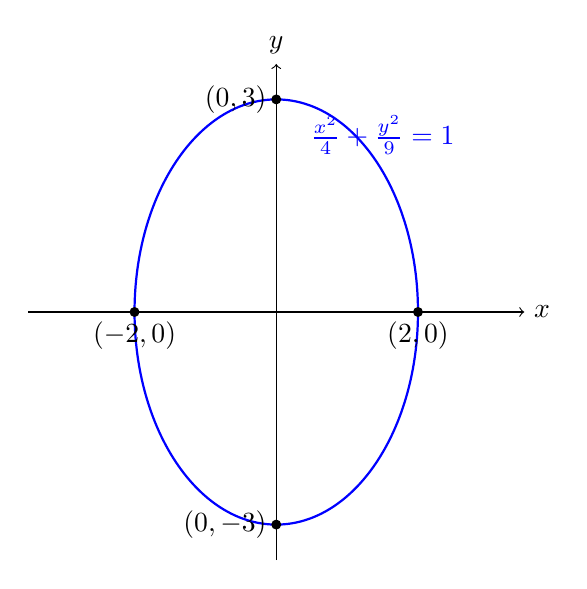
\begin{tikzpicture}[scale=0.9]
    % Axes
    \draw[->] (-3.5,0) -- (3.5,0) node[right] {$x$};
    \draw[->] (0,-3.5) -- (0,3.5) node[above] {$y$};

    % Ellipse: x^2/4 + y^2/9 = 1
    \draw[thick, blue] (0,0) ellipse (2 and 3);

    % Mark key points
    \foreach \x in {-2,2} \fill (\x,0) circle (2pt) node[below] {$(\x,0)$};
    \foreach \y in {-3,3} \fill (0,\y) circle (2pt) node[left] {$(0,\y)$};

    % Label the curve
    \node[blue] at (1.5,2.5) {$\frac{x^2}{4} + \frac{y^2}{9} = 1$};
\end{tikzpicture}
\end{center}

\begin{tcolorbox}[title=Problem 8, breakable]
    \[C = \left\{(x, y) \in \mathbb{R}^2 \mid x^2 - y^2 - 4 = 0\right\}.\]
    Show that if $(x, y) \in C$, then the three points $(-x, y), (x, -y)$, and $(-x, -y)$
    are also on $C$. Thus the curve $C$ is also symmetric about the $x-$ and $y$-axes.
\end{tcolorbox}

\begin{proof}
    Let $(x, y) \in \mathbb{R}^2$.
    Suppose $x^2 - y^2 - 4 = 0$.
    Notice that $x^2 = (-x)^2$ and $y = (-y)^2$. Then 
    \[x^2 - y^2 - 4 = (-x)^2 - y^2 = x^2 - (-y)^2 = (-x)^2 - (-y)^2 = 0.\]
    Thus $(-x, y), (x, -y), (-x, -y) \in C$.
\end{proof}

\begin{tcolorbox}[title=Problem 9, breakable]
    \[C = \left\{(x, y) \in \mathbb{R}^2 \mid x^2 - y^2 - 4 = 0\right\}.\]
    Show that if $(x, y) \in C$, then we have $|x| \ge 2$.
\end{tcolorbox}

\begin{proof}
    Let $(x, y) \in \mathbb{R}^2$.
    Suppose $x^2 - y^2 - 4 = 0$.
    Then 
    \[x^2 - y^2 - 4 = 0 \iff x^2 = y^2 + 4 \iff |x| = \sqrt{y^2 + 4} \ge \sqrt{4} = 2.\]
\end{proof}

\begin{tcolorbox}[title=Problem 10, breakable]
    \[C = \left\{(x, y) \in \mathbb{R}^2 \mid x^2 - y^2 - 4 = 0\right\}.\]
    Show that the curve $C$ is unbounded in the positive 
        and negative $x$-directions and also unbounded in the 
        positive and negative $y$-directions.
\end{tcolorbox}

\begin{proof}
    First notice
    \[
        x^2 - y^2 - 4 = 0 
        \iff x^2 = y^2 + 4 
        \iff x = \pm \sqrt{y^2 + 4}
        \iff y = \pm \sqrt{x^2 - 4}.
    \]
    As $y \to \infty$, we have $x = \pm \sqrt{y^2 + 4} \to \infty$ and $-\infty$.
    Similarly, as $x \to \infty$, we have $y = \pm \sqrt{x^2 - 4} \to \infty$ and $-\infty$.
\end{proof}


\begin{tcolorbox}[title=Problem 11, breakable]
    Sketch 
    \[C = \left\{(x, y) \in \mathbb{R}^2 \mid x^2 - y^2 - 4 = 0\right\}.\]
\end{tcolorbox}

\begin{center}
\begin{tikzpicture}[scale=0.8]
    % Axes
    \draw[->] (-6,0) -- (6,0) node[right] {$x$};
    \draw[->] (0,-5) -- (0,5) node[above] {$y$};

    % Hyperbola x^2 - y^2 = 4
    \draw[domain=-5:-2, smooth, thick, blue] 
        plot (\x, {sqrt(\x*\x - 4)});
    \draw[domain=-5:-2, smooth, thick, blue] 
        plot (\x, {-sqrt(\x*\x - 4)});
    \draw[domain=2:5, smooth, thick, blue] 
        plot (\x, {sqrt(\x*\x - 4)});
    \draw[domain=2:5, smooth, thick, blue] 
        plot (\x, {-sqrt(\x*\x - 4)});

    % Asymptotes y = ±x
    \draw[dashed] (-5,-5) -- (5,5);
    \draw[dashed] (-5,5) -- (5,-5);

    % Label
    \node[blue] at (3.5,2.5) {$x^2 - y^2 = 4$};
\end{tikzpicture}
\end{center}

\begin{tcolorbox}[title=Problem 12, breakable]
    Sketch the graph of each of the following conics in 
        $\mathbb{R}^2$.
    Identify which are parabolas, ellipses, or Hyperbola.
    \begin{enumerate}
        \item $V(x^2 - 8y)$.
        \item $V(x^2 + 2x - y^2 - 3y - 1)$.
        \item $V(4x^2 + y^2)$.
        \item $V(3x^2 + 3y^2 - 75)$.
        \item $V(x^2 - 9y^2)$.
        \item $V(4x^2 + y^2 - 8)$.
        \item $V(x^2 + 9y^2 - 36)$.
        \item $V(x^2 - 4 y^2 - 16)$.
        \item $V(y^2 - x^2 - 9)$.
    \end{enumerate}
\end{tcolorbox}

\textbf{Solution (1):}
Parabola.
\begin{figure}[h!]
    \centering
    \includegraphics[width=0.3\textwidth]{images/chapter1/1.png}
\end{figure}

\textbf{Solution (2):}
Hyperbola.
\begin{figure}[h!]
    \centering
    \includegraphics[width=0.3\textwidth]{images/chapter1/2.png}
\end{figure}

\textbf{Solution (3):}
Point.

\textbf{Solution (4):}
Ellipse.
\begin{figure}[h!]
    \centering
    \includegraphics[width=0.3\textwidth]{images/chapter1/4.png}
\end{figure}

\textbf{Solution (5):}
Two lines.
\begin{figure}[h!]
    \centering
    \includegraphics[width=0.3\textwidth]{images/chapter1/5.png}
\end{figure}

\textbf{Solution (6):}
Ellipse.
\begin{figure}[h!]
    \centering
    \includegraphics[width=0.3\textwidth]{images/chapter1/6.png}
\end{figure}

\textbf{Solution (7):}
Ellipse.
\begin{figure}[h!]
    \centering
    \includegraphics[width=0.3\textwidth]{images/chapter1/7.png}
\end{figure}

\textbf{Solution (8):}
Hyperbola.
\begin{figure}[h!]
    \centering
    \includegraphics[width=0.3\textwidth]{images/chapter1/8.png}
\end{figure}

\textbf{Solution (9):}
Hyperbola.
\begin{figure}[h!]
    \centering
    \includegraphics[width=0.3\textwidth]{images/chapter1/9.png}
\end{figure}

\begin{tcolorbox}[title=Problem 13, breakable]
    Express the polynomial $P(x, y) = ax^2 + bxy + cy^2 + dx + ey + h$ in the form
    \[P(x, y) = Ax^2 + Bx + C,\]
    where $A, B$, and $C$ are polynomials in $y$. What are $A, B$, and $C$?
\end{tcolorbox}

\begin{proof}
    Let $A = a, B = by + d$, and $C = cy^2 + ey + h$.
    Notice 
    \[
    ax^2 + bxy + cy^2 + dx + ey + h
    = a x^2 + bxy + dx + cy^2 + ey + h
    = a x^2 + (by + d)x + (cy^2 + ey + h)
    = Ax^2 + Bx + C.
    \]
\end{proof}

\begin{tcolorbox}[title=Problem 14, breakable]
    Treating $P(x, y) = ax^2 + bxy + cy^2 + dx + cy + h$ as a polynomial
    in the variable $x$, show that the discriminant is 
    \[\triangle_x (y) = (b^2 - 4ac)y^2 + (2bd - 4ae)y + (d^2 - 4ah).\]
\end{tcolorbox}

\begin{proof}
    From Problem 13 we have $A = a, B = by + d$, and $C = cy^2 + ey + h$.
    Then 
    \[
    \triangle_x (y) = B^2 - 4AC
    = (by + d)^2 - 4a(cy^2 + ey + h)
    = (b^2 - 4ac)y^2 + (2bd - 4ae)y + (d^2 - 4ah).
    \]
\end{proof}

\begin{tcolorbox}[title=Problem 15, breakable]
    \begin{enumerate}
        \item Suppose $\triangle_x (y_0) < 0$. Explain why there is no point on $V(p)$ whose $y$-coordinate is $y_0$.
        \item Suppose $\triangle_x (y_0) = 0$. Explain why there is exactly one point on $V(P)$ whose $y$-coordinate is $y_0$.
        \item Suppose $\triangle_x (y_0) > 0$. Explain why there are exactly two points on $V(P)$ whose $y$-coordinate is $y_0$.
    \end{enumerate}
\end{tcolorbox}

\textbf{Solution (a):} In $\mathbb{R}$, the square root is undefined for values $< 0$.

\textbf{Solution (b):} If $\triangle_x (y_0) = 0$, then $+\sqrt{B^2 - 4AC} = -\sqrt{B^2 - 4AC}$,  
so there is exactly one point on $V(P)$ whose $y$-coordinate is $y_0$.

\textbf{Solution (c):} If $\triangle_x (y_0) > 0$, then $+\sqrt{B^2 - 4AC} \ne -\sqrt{B^2 - 4AC}$,  
so there are exactly two points on $V(P)$ whose $y$-coordinate is $y_0$.

\newpage
\begin{tcolorbox}[title=Problem 16, breakable]
    Suppose $b^2 - 4ac = 0$. Suppose further that $2bd - 4 ae > 0$.
    \begin{enumerate}
        \item Show that $\triangle_x (y) \ge 0$ if and only if $y \ge \frac{4 ah - d^2}{2bd - 4ae}$.
        \item Conclude that if $b^2 - 4ac = 0$ and $2bd - 4ae > 0$, then $V(P)$ is a parabola.
    \end{enumerate}
\end{tcolorbox}

\begin{proof}
    Suppose $\triangle_x (y) \ge 0$.
    Then 
    \begin{align*}
        \triangle_x (y) &= (b^2 - 4ac)y^2 + (2bd - 4ae)y + (d^2 - 4ah) \\
                        &= 0 y^2 + (2bd - 4 ae)y + (d^2 - 4ah).
    \end{align*}
    Therefore,
    \[
        (2bd - 4ae)y + (d^2 - 4ah) \ge 0.
    \]
    Since $2bd - 4ae > 0$, we have
    \[
        y \ge \frac{4ah - d^2}{2bd - 4ae}.
    \]

    Conversely, suppose $y \ge \frac{4ah - d^2}{2bd - 4ae}$.
    Then 
    \begin{align*}
        \triangle_x (y) &= (2bd - 4ae)y + (d^2 - 4ah) \\
                        &\ge (2bd - 4ae)\left(\frac{4ah - d^2}{2bd - 4ae}\right) + (d^2 - 4ah) \\
                        &= 0.
    \end{align*}
\end{proof}

\begin{proof}
    Suppose $b^2 - 4ac = 0$ and $2bd - 4ae > 0$.
    Then $\triangle_x (y) = (2bd - 4ae)y + (d^2 - 4ah)$.
    Now, $x = \frac{-B \pm \sqrt{B^2 - 4AC}}{2A}$.
    It is clear that $x$ is symmetrical, and since $y \ge \frac{4ah - d^2}{2bd - 4ae}$,
    $V(P)$ is a parabola.
\end{proof}

\begin{tcolorbox}[title=Problem 17, breakable]
    Suppose $b^2 - 4ac < 0$.
    \begin{enumerate}
        \item Show that one of the following occurs:
        \begin{enumerate}
            \item $\{y \mid \triangle_x (y) \ge 0\} = \emptyset$,
            \item $\{y \mid \triangle_x (y) \ge 0\} = \{y_o\}$,
            \item there exist real numbers $\alpha$ and $\beta$, $\alpha < \beta$, such that 
            \[\{y \mid \triangle_x (y) \ge 0\} = \{y \mid \alpha \le y \le \beta\}.\]
        \end{enumerate}
        \item Conclude that $V(P)$ is either emptyset, a point, or an ellipse.
    \end{enumerate}
\end{tcolorbox}

\begin{proof}
    We can compare the quadratic term $(b^2 - 4ac)y^2 \le 0$ with the linear 
        term $(2bd - 4ae)y + (d^2 - 4ah)$ in $\triangle_x (y)$.
    There are three cases depending on whether the linear term 
        intersects the quadratic term zero, once, or twoice.
\end{proof}

\begin{tcolorbox}[title=Problem 18, breakable]
\end{tcolorbox}

\begin{tcolorbox}[title=Problem 19, breakable]
\end{tcolorbox}